\subsection{Random Forests}

A random forest was computed in figure \ref{fig:success_time_vs_trees_randomForest} using G3M2 data as test set and the remaining 14 students as train set.
The number of trees was varied and the time measured.

\begin{figure}[H]
\centering
\includegraphics[width = 0.95 \textwidth]{graphics/successRate_randomForest}
\caption{Success rate and time taken to compute the trees needed in the random forest as the number of trees increases.}
\label{fig:success_time_vs_trees_randomForest}
\end{figure}

As can be seen on figure \ref{fig:success_time_vs_trees_randomForest}, then the success rate increases drastically from 0 to 500 trees in the random forest where it settles around 67\%.
The time increases linearly with the number of trees, but with some inconsistencies towards the end.

From figure \ref{fig:success_time_vs_trees_randomForest} it was decided to use 200 trees for the optimum random forest.
Figure \ref{fig:success_randomForest} was generated using the 200 trees.
Each point was computed using the a single person in the test set and independently the 14 other in the training set.

% 0.37700 0.44475 0.35250 0.51550 0.42025 0.43425 0.45750 0.60900 0.63775 0.43525 0.46500 0.55750 0.54525 0.47625 0.29200
\begin{figure}[H]
\centering
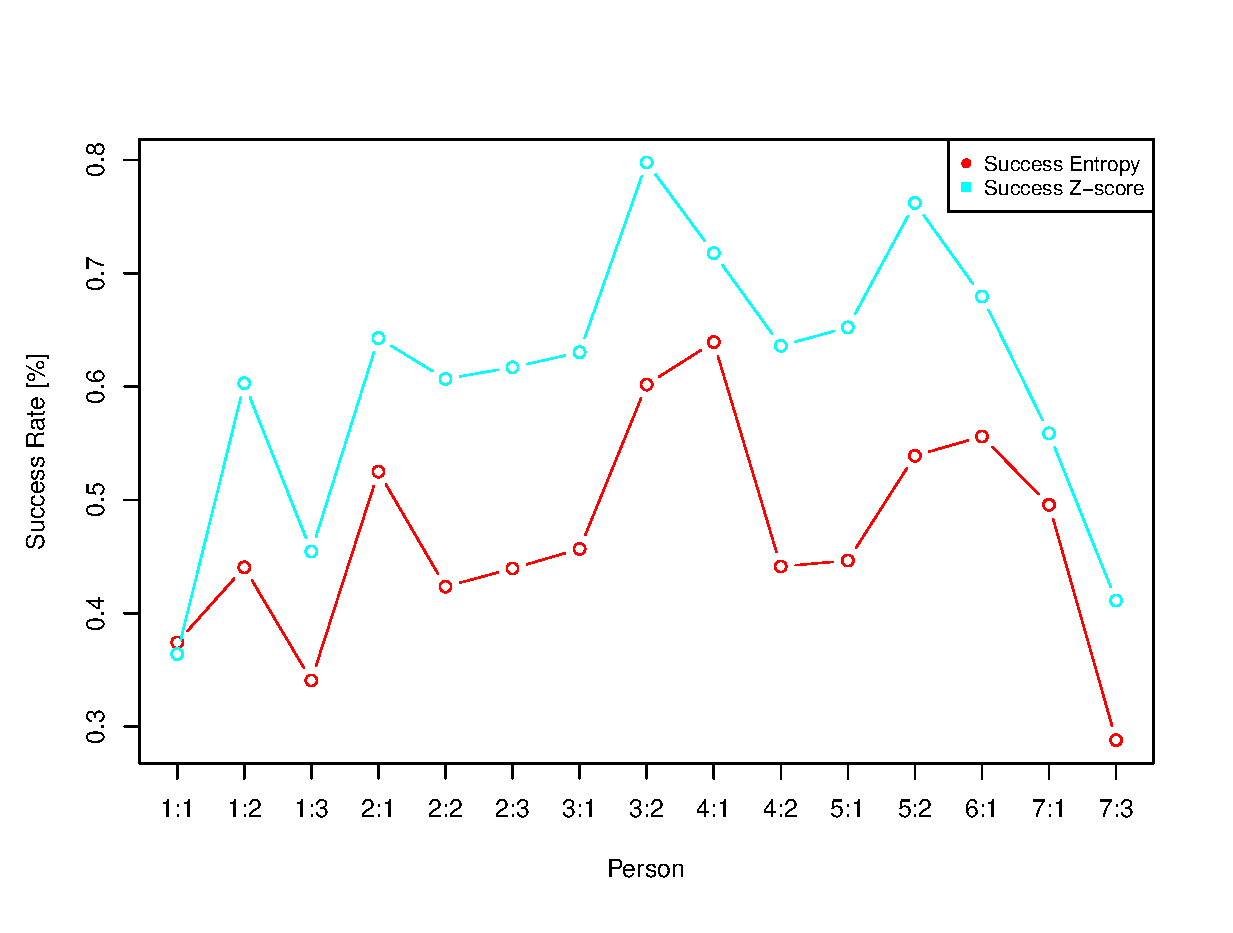
\includegraphics[width = 0.95 \textwidth]{graphics/successRate_randomForest_comp}
\caption{Success rate for the different people given they are not present in the data set. The mean success rate is 46.8\%.}
\label{fig:success_randomForest}
\end{figure}